%{{第六十六回}}{第六十六回}}

\chapter{情小妹耻情归地府\\冷二郎一冷入空门}

{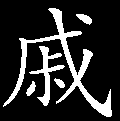
\includegraphics[width=3mm]{../Images/00005}\kaishu 余叹世人不识``情''字,常把``淫''字当作``情''字。殊不知淫里无情,情里无淫,淫必伤情,情必戒淫,情断处淫生,淫断处情生。三姐项下一横,是绝情,乃是正情;湘莲万根皆削,是无情,乃是至情。生为情人,死为情鬼。故结句曰``来自情天,去自情地'',岂非一篇尽情文字?再看他书,则全是``淫''不是``情''了。}

话说鲍二家的走来打了兴儿一下子,笑道:``原有些真的,叫你又编了这混话,越发没了捆儿了。你倒不像跟二爷的人,这些混话倒像是宝玉那边的了。''{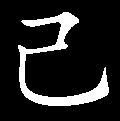
\includegraphics[width=3mm]{../Images/00003}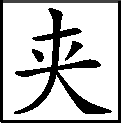
\includegraphics[width=3mm]{../Images/00012}\footnotesize \kaishu 好极之文,将茗烟等已全写出,可谓一击两鸣法,不写之写也。}尤二姐才要又问,忽见尤三姐笑问道:``可是你们家那宝玉,除了上学,他作些什么?''{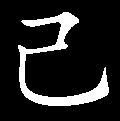
\includegraphics[width=3mm]{../Images/00003}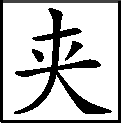
\includegraphics[width=3mm]{../Images/00012}\footnotesize \kaishu 拍案叫绝!此处方问,是何文情!}

兴儿笑道:``姨娘别问他,说起来姨娘也未必信。他长了这么大,独他没有上过正经学堂。我们家从祖宗直到二爷,谁不是寒窗十载,偏他不喜读书。老太太的宝贝,老爷先还管,如今也不敢管了。成天家疯疯颠颠的,说的话人也不懂,干的事人也不知。外头人人看着好清俊模样儿,心里自然是聪明的,谁知是外清而内浊,见了人,一句话也没有。所有的好处,虽没上过学,倒难为他认得几个字。每日也不习文,也不学武,又怕见人,只爱在丫头群里闹。再者也没刚柔,有时见了我们,喜欢时没上没下,大家乱顽一阵;不喜欢各自走了,他也不理人。我们坐着卧着,见了他也不理,他也不责备。因此没人怕他,只管随便,都过的去。''

尤三姐笑道:``主子宽了,你们又这样;严了,又抱怨。可知难缠。''{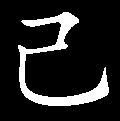
\includegraphics[width=3mm]{../Images/00003}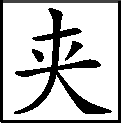
\includegraphics[width=3mm]{../Images/00012}\footnotesize \kaishu 情语,情文至语。}尤二姐道:``我们看他倒好,原来这样。可惜了一个好胎子。''尤三姐道:``姐姐信他胡说,咱们也不是见一面两面的,行事言谈吃喝,原有些女儿气,那是只在里头惯了的。若说糊涂,那些儿糊涂?姐姐记得,穿孝时咱们同在一处,那日正是和尚们进来绕棺,咱们都在那里站着,他只站在头里挡着人。人说他不知礼,又没眼色。过后他没悄悄的告诉咱们说:`\elegantpar{姐姐不知道,我并不是没眼色。想和尚们脏,恐怕气味熏了姐姐们。}{尽心平儿一节}''接着他吃茶,姐姐又要茶,那个老婆子就拿了他的碗倒。他赶忙说:``我吃脏了的,另洗了再拿来。'这两件上,我冷眼看去,原来他在女孩子们前不管怎样都过的去,只不大合外人的式,所以他们不知道。''尤二姐听说,笑道:``依你说,你两个已是情投意合了。竟把你许了他,岂不好?''三姐见有兴儿,不便说话,只低头嗑瓜子。兴儿笑道:``若论模样儿行事为人,倒是一对好的。只是他已有了,只未露形。将来准是林姑娘定了的。因林姑娘多病,二则都还小,故尚未及此。\elegantpar{再过三二年,老太太便一开言,那是再无不准的了。}{没这么好命}''大家正说话,只见隆儿又来了,说:``老爷有事,是件机密大事,要遣二爷往平安州去。不过三五日就起身,来回也得半月工夫。今日不能来了。请老奶奶早和二姨定了那事,明日爷来,好作定夺。''说着,带了兴儿回去了。

这里尤二姐命掩了门早睡,盘问他妹子一夜。至次日午后,贾琏方来了。尤二姐因劝他说:``既有正事,何必忙忙又来,千万别为我误事。''贾琏道:``也没甚事,只是偏偏的又出来了一件远差。出了月就起身,得半月工夫才来。''尤二姐道:``既如此,你只管放心前去,这里一应不用你记挂。三妹子他从不会朝更暮改的。他已说了改悔,必是改悔的。他已择定了人,你只要依他就是了。''贾琏问是谁,尤二姐笑道:``这人此刻不在这里,不知多早才来,也难为他眼力。自己说了,这人一年不来,他等一年;十年不来,等十年;若这人死了再不来了,他情愿剃了头当姑子去,吃长斋念佛,以了今生。''贾琏问:``到底是谁,这样动他的心?''二姐笑道:``说来话长。五年前我们老娘家里做生日,妈和我们到那里与老娘拜寿。他家请了一起串客,里头有个作小生的叫作柳湘莲,{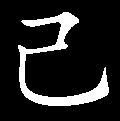
\includegraphics[width=3mm]{../Images/00003}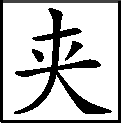
\includegraphics[width=3mm]{../Images/00012}\footnotesize \kaishu 千奇百怪之文,何至于此!}他看上了,如今要是他才嫁。旧年我们闻得柳湘莲惹了一个祸逃走了,不知可有来了不曾?''贾琏听了道:``怪道呢!我说是个什么样人,原来是他!果然眼力不错。你不知道这柳二郎,那样一个标致人,最是冷面冷心的,差不多的人,都无情无义。他最和宝玉合的来。\elegantpar{去年因打了薛呆子}{打得好},他不好意思见我们的,不知那里去了一向。后来听见有人说来了,不知是真是假,一问宝玉的小子们就知道了。倘或不来,他萍踪浪迹,知道几年才来,岂不白耽搁了?''尤二姐道:``我们这三丫头说的出来,干的出来,他怎样说,只依他便了。''

二人正说之间,只见尤三姐走来说道:``姐夫,你只放心。我们不是那心口两样人,说什么是什么。若有了姓柳的来,我便嫁他。从今日起,我吃斋念佛,只伏侍母亲,等他来了,嫁了他去,若一百年不来,我自己修行去了。''说着,将一根玉簪,击作两段,``一句不真,就如这簪子!''说着,回房去了,真个竟非礼不动,非礼不言起来。贾琏无了法,只得和二姐商议了一回家务,复回家与凤姐商议起身之事。一面着人问茗烟,茗烟说:``竟不知道。大约未来;若来了,必是我知道的。''一面又问他的街坊,也说未来。贾琏只得回复了二姐。至起身之日已近,前两天便说起身,却先往二姐这边来住两夜,从这里再悄悄长行。果见小妹竟又换了一个人,又见二姐持家勤慎,自是不消记挂。

是日一早出城,就奔平安州大道,晓行夜住,渴饮饥餐。方走了三日,那日正走之间,顶头来了一群驮子,内中一夥,主仆十来骑马,走的近来一看,不是别人,竟是薛蟠和柳湘莲来了。贾琏深为奇怪,{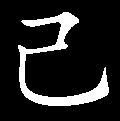
\includegraphics[width=3mm]{../Images/00003}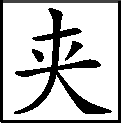
\includegraphics[width=3mm]{../Images/00012}\footnotesize \kaishu 余亦为怪。}忙伸马迎了上来,大家一齐相见,说些别后寒温,大家便入酒店歇下,叙谈叙谈。贾琏因笑说:``闹过之后,我们忙着请你两个和解,谁知柳兄踪迹全无。怎么你两个今日倒在一处了?''薛蟠笑道:``天下竟有这样奇事。我同伙计贩了货物,自春天起身,往回里走,一路平安。谁知前日到了平安州界,遇一伙强盗,已将东西劫去。不想柳二弟从那边来了,方把贼人赶散,夺回货物,还救了我们的性命。我谢他又不受,所以我们结拜了生死弟兄,如今一路进京。从此后我们是亲弟亲兄一般。到前面岔口上分路,他就分路往南二百里有他一个姑妈,他去望候望候。我先进京去安置了我的事,然后给他寻一所宅子,寻一门好亲事,大家过起来。''贾琏听了道:``原来如此,倒教我们悬了几日心。''因又听道寻亲,又忙说道:``我正有一门好亲事堪配二弟。''说着,便将自己娶尤氏,如今又要发嫁小姨一节说了出来,只不说尤三姐自择之语。又嘱薛蟠且不可告诉家里,等生了儿子,自然是知道的。

薛蟠听了大喜,说:``早该如此,这都是\elegantpar{舍表妹}{这里指谁}之过。''湘莲忙笑说:``你又忘情了,还不住口。''薛蟠忙止住不语,便说:``既是这等,这门亲事定要做的。''湘莲道:``我本有愿,定要一个绝色的女子。如今既是贵昆仲高谊,顾不得许多了,任凭裁夺,我无不从命。''贾琏笑道:``如今口说无凭,等柳兄一见,便知我这内娣的品貌是古今有一无二的了。''湘莲听了大喜,说:``既如此说,等弟探过姑娘,不过月中就进京的,那时再定如何?''贾琏笑道:``你我一言为定,只是我信不过柳兄。你乃是萍踪浪迹,倘然淹滞不归,岂不误了人家。须得留一定礼。''湘莲道:``大丈夫岂有失信之理。小弟素系寒贫,况且客中,何能有定礼。''薛蟠道:``我这里现成,就备一分二哥带去。''贾琏笑道:``也不用金帛之礼,须是柳兄亲身自有之物,不论物之贵贱,不过我带去取信耳。''湘莲道:``既如此说,弟无别物,此剑防身,不能解下。囊中尚有一把鸳鸯剑,乃吾家传代之宝,弟也不敢擅用,只随身收藏而已。贾兄请拿去为定。弟纵系水流花落之性,然亦断不舍此剑者。''说毕,\href{../Text/part0070_split_000.html\#lnkback_1_a}{\textsuperscript{①}}大家又饮了几杯,方各自上马。作别起程。正是:

将军不下马,各自奔前程。

且说贾琏一日到了平安州,见了节度,完了公事。因又嘱他十月前后务要还来一次,贾琏领命。次日连忙取路回家,先到尤二姐处探望。谁知贾琏出门之后,尤二姐操持家务十分谨肃,每日关门合户,一点外事不闻。他小妹子果是个斩钉截铁之人,每日侍奉母姊之馀,只安分守已,随分过活。虽是夜晚间孤衾独枕,不惯寂寞,奈一心丢了众人,只念柳湘莲早早回来完了终身大事。这日贾琏进门,见了这般景况,喜之不尽,深念二姐之德。大家叙些寒温之后,贾琏便将路上相遇湘莲一事说了出来,又将鸳鸯剑取出,递与三姐。三姐看时,上面龙吞夔护,珠宝晶莹,将靶一掣,里面却是两把合体的。一把上面錾着一``鸳''字,一把上面錾着一``鸯''字,冷飕飕,明亮亮,如两痕秋水一般。三姐喜出望外,连忙收了,挂在自己绣房床上,每日望着剑,自笑终身有靠。贾琏住了两天,回去复了父命,回家合宅相见。那时凤姐已大愈,出来理事行走了。贾琏又将此事告诉了贾珍。贾珍因\elegantpar{近日又遇了新友}{又是谁},将这事丢过,不在心上,任凭贾琏裁夺,只怕贾琏独力不加,少不得又给了他三十两银子。贾琏拿来交与二姐预备妆奁。

谁知八月内湘莲方进了京,先来拜见薛姨妈,又遇见薛蝌,方知薛蟠不惯风霜,不服水土,一进京时便病倒在家,请医调治。听见湘莲来了,请入卧室相见。薛姨妈也不念旧事,只感新恩,母子们十分称谢。又说起亲事一节,凡一应东西皆已妥当,只等择日。柳湘莲也感激不尽。

次日又来见宝玉,二人相会,如鱼得水。湘莲因问贾琏偷娶二房之事,宝玉笑道:``我听见茗烟一干人说,我却未见,我也不敢多管。我又听见茗烟说,琏二哥哥着实问你,不知有何话说?''湘莲就将路上所有之事一概告诉宝玉,宝玉笑道:``大喜,大喜!难得这个标致人,果然是个古今绝色,堪配你之为人。''湘莲道:``既是这样,他那里少了人物,如何只想到我。况且我又素日不甚和他厚,也关切不至此。路上工夫忙忙的就那样再三要来定,难道女家反赶着男家不成。我自己疑惑起来,后悔不该留下这剑作定。所以后来想起你来,可以细细问个底里才好。''宝玉道:``你原是个精细人,如何既许了定礼又疑惑起来?你原说只要一个绝色的,如今既得了个绝色便罢了,何必再疑?''湘莲道:``你既不知他娶,如何又知是绝色?''宝玉道:``\elegantpar{他是珍大嫂子的继母带来的两位小姨。}{方知二姐三姐由来}我在那里和他们混了一个月,怎么不知?真真一对尤物,{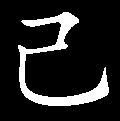
\includegraphics[width=3mm]{../Images/00003}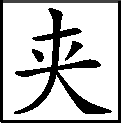
\includegraphics[width=3mm]{../Images/00012}\footnotesize \kaishu 可巧。}他又姓尤。''湘莲听了,跌足道:``这事不好,断乎做不得了。\elegantpar{你们东府里除了那两个石头狮子干净,只怕连猫儿狗儿都不干净。我不做这剩忘八。}{转世成功,头上有人摸着,说道“只有这石狮子还算干净”}''{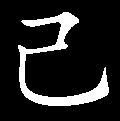
\includegraphics[width=3mm]{../Images/00003}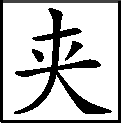
\includegraphics[width=3mm]{../Images/00012}\footnotesize \kaishu 极奇之文!极趣之文!《金瓶梅》中有云``把忘八的脸打绿了'',已奇之至,此云``剩忘八'',岂不更奇!}宝玉听说,红了脸。湘莲自惭失言,连忙作揖说:``我该死胡说。{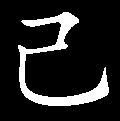
\includegraphics[width=3mm]{../Images/00003}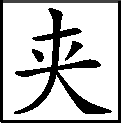
\includegraphics[width=3mm]{../Images/00012}\footnotesize \kaishu 忽用湘莲提东府之事,骂及宝玉,可是人想得到的?所谓``一个人不曾放过''。}你好歹告诉我,他品行如何?''宝玉笑道:``你既深知,又来问我作甚么?连我也未必干净了。''湘莲笑道:``原是我自己一时忘情,好歹别多心。''宝玉笑道:``何必再提,这倒似有心了。''湘莲作揖告辞出来,若去找薛蟠,一则他现卧病,二则他又浮躁,不如去索回定礼。主意已定,便一径来找贾琏。

贾琏正在新房中,闻得湘莲来了,喜之不禁,忙迎了出来,让到内室与尤老相见。湘莲只作揖称老伯母,自称晚生,贾琏听了诧异。吃茶之间,湘莲便说:``客中偶然忙促,谁知家姑母于四月间订了弟妇,使弟无言可回。若从了老兄背了姑母,似非合理。若系金帛之订,弟不敢索取,但此剑系祖父所遗,请仍赐回为幸。''贾琏听了,便不自在,还说:``定者,定也。原怕反悔所以为定。岂有婚姻之事,出入随意的?还要斟酌。''湘莲笑道:``虽如此说,弟愿领责领罚,然此事断不敢从命。''贾琏还要饶舌,湘莲便起身说:``请兄外坐一叙,此处不便。''那尤三姐在房明明听见。好容易等了他来,今忽见反悔,便知他在贾府中得了消息,自然是嫌自己淫奔无耻之流,不屑为妻。今若容他出去和贾琏说退亲,料那贾琏必无法可处,自己岂不无趣。一听贾琏要同他出去,连忙摘下剑来,将一股雌锋隐在肘内,出来便说:``你们不必出去再议,还你的定礼。''一面泪如雨下,左手将剑并鞘送与湘莲,右手回肘只往项上一横。可怜------

揉碎桃花红满地,玉山倾倒再难扶。

芳灵蕙性,渺渺冥冥,不知那边去了。当下唬得众人急救不迭。尤老一面嚎哭,一面又骂湘莲。贾琏忙揪住湘莲,命人捆了送官。尤二姐忙止泪反劝贾琏:``你太多事,人家并没威逼他死,是他自寻短见。你便送他到官,又有何益,反觉生事出丑。不如放他去罢,岂不省事。''贾琏此时也没了主意,便放了手命湘莲快去。湘莲反不动身,泣道:``\elegantpar{我并不知是这等刚烈贤妻}{金陵十三钗不知严歌苓和张艺谋之间的区别},可敬,可敬。''湘莲反扶尸大哭一场。等买了棺木,眼见入殓,又俯棺大哭一场,方告辞而去。

出门无所之,昏昏默默,自想方才之事。原来尤三姐这样标致,又这等刚烈,自悔不及。正走之间,只见薛蟠的小厮寻他家去,那湘莲只管出神。那小厮带他到新房之中,十分齐整。忽听环佩叮当,尤三姐从外而入,一手捧着鸳鸯剑,一手捧着一卷册子,向柳湘莲泣道:``妾痴情待君五年矣,不期君果冷心冷面,妾以死报此痴情。妾今奉警幻之命,前往太虚幻境修注案中所有一干情鬼。妾不忍一别,故来一会,从此再不能相见矣。''说着便走。湘莲不舍,忙欲上来拉住问时,那尤三姐便说:``来自情天,去由情地。前生误被情惑,今既耻情而觉,与君两无干涉。''说毕,一阵香风,无踪无影去了。

湘莲警觉,似梦非梦,睁眼看时,那里有薛家小童,也非新室,竟是一座破庙,旁边坐着一个跏腿道士捕虱。湘莲便起身稽首相问:``此系何方?仙师仙名法号?''道士笑道:``连我也不知道此系何方,我系何人,不过暂来歇足而已。''柳湘莲听了,不觉冷然如寒冰侵骨,\elegantpar{掣出那股雄剑,将万根烦恼丝一挥而尽}{剑法高明},便随那道士,不知往那里去了。后回便见。

{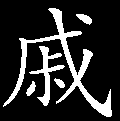
\includegraphics[width=3mm]{../Images/00005}\kaishu 总评:尤三姐失身时,浓妆艳抹凌辱群凶;择夫后,念佛吃斋敬奉老母;能辨宝玉能识湘莲,活是红拂文君一流人物。}

{\kaishu 鸳鸯剑能斩鸳鸯,鸳鸯人能破鸳鸯,岂有此理?鸳鸯剑梦里不会杀奸妇,鸳鸯人白日偏要助淫夫,焉有此情?真天地间不测的怪事!}

% {\href{../Text/part0070_split_000.html\#navto_1_a}{①}此处列本比诸本独多``解囊出剑捧与贾琏,贾琏命人收了。''两句,交代的清楚明白。不过这不像作者的行文风格。}

